% PoPETs submission format (acmart, sigconf, double-blind review mode).
% Figures and tables are generated by script from reports/ -- see
% paper/scripts/generate_figures.py and generate_plots.py. Do not
% hand-edit generated tables/figures; edit the source report and
% regenerate instead.
\documentclass[sigconf,review,anonymous]{acmart}

\acmConference[PoPETs]{Proceedings on Privacy Enhancing Technologies}{}{}
\settopmatter{printacmref=false}
\renewcommand\footnotetextcopyrightpermission[1]{}
\pagestyle{plain}

\usepackage{booktabs}
\usepackage{graphicx}

\begin{document}

\title{Who Is Actually Protected? Learned Mobility Privacy Leaves the Most Identifiable Users Exposed}

\begin{abstract}
Learned mobility-privacy mechanisms are typically evaluated by training
once, attacking the output with a single group-agnostic adversary, and
reporting an aggregate privacy gain. We show this protocol hides a
systematic disparity: using a PyTorch reimplementation and audit of a
representative mechanism (``Mo-PAE'', studied here in the third person
as prior work under double-blind review), the lowest-entropy decile of
users -- the most routine, most behaviorally predictable, and so the
most identifiable to begin with -- consistently receives the smallest
relative risk reduction of any decile and is left with a residual
re-identification risk 2--9$\times$ higher than the best-protected
decile, a disparity that is statistically robust across three real
mobility datasets (GeoLife, Foursquare, four Gowalla metro subsets) and
survives standard regression controls. Adding an explicit fairness term
to the training objective does not reliably fix this: across the
formulations we test, raising the fairness weight either leaves the
most-identifiable decile's risk unchanged while protecting an
already-better-off decile further, or trades utility for risk reduction
without closing the gap -- no formulation we test is shown to dominate
the undefended mechanism once both training convergence and
encoder-initialization variance are properly controlled. We further
show that a large class of adaptive adversaries previously thought to
exploit this unevenness more aggressively than a naive attacker derive
almost all of their apparent advantage from a smaller candidate pool
and oracle knowledge of a user's behavioral group, not from genuine
attacker sophistication -- a realistic adaptive adversary without that
side information performs no better, and often worse, than a naive one.
Together, these results indicate that a learned mobility-privacy
mechanism's own evaluation protocol can systematically understate risk
for exactly the users who most need protection, and that closing this
gap requires measuring and targeting it directly, not assuming an
aggregate privacy objective will do so as a side effect.
\end{abstract}

\maketitle

\section{Introduction}
\label{sec:intro}

The proliferation of mobile devices and location-based services has
produced an abundance of spatial-temporal mobility data, which in turn
enables applications in urban planning~\cite{zheng2014urban,
jayarajah2018understanding}, transportation-equity analysis, contagious
disease management~\cite{eubank2004modelling,
wesolowski2012quantifying, ghadiri2024recreational}, and next-location
prediction more broadly~\cite{luca2021survey}. These same mobility
traces pose serious re-identification risk, since individuals are often
identifiable from their movement patterns
alone~\cite{de2013unique, saleheen2016msieve}. Privacy-utility trade-off
(PUT) models learn representations that preserve downstream utility
while suppressing re-identifiability, but prior work evaluating such
models has found that they can satisfy \emph{group} fairness checks
while violating \emph{individual} fairness -- treating users with
similar mobility behavior very differently in how much privacy
protection they actually receive~\cite{zhan2023analysing}. Equity
analysis in transportation research has traditionally relied on
coarser, demographic or region-level disparity
measures~\cite{yan2020fairness, yan2019fairst, he2025framework}; this
paper instead asks the question at the level of the individual user,
following the individual-fairness principle that similar individuals
should receive similar treatment~\cite{dwork2012fairness}.

A learned mobility-privacy mechanism is typically evaluated by training
it once, attacking its output with a single, group-agnostic
re-identification attacker, and reporting an aggregate or per-group
privacy gain. This paper asks a narrower question than ``is the
mechanism private'': \emph{who, specifically, is protected, and does
the mechanism's own evaluation protocol correctly report that}? If this
question is answered with an unreliable measurement protocol, a
mechanism can appear equitable while in fact systematically
under-protecting exactly the users most in need of protection.

We study this question on a representative learned mechanism from the
mobility-privacy literature, referred to throughout this paper in the
third person as Mo-PAE~\cite{zhan2023mopae} (an encoder/decoder/adversary
architecture that trains a feature encoder adversarially against an
in-model re-identification head, following the published PETS 2023
design this project audited and reimplemented in PyTorch).

\textbf{Contributions.} This paper makes four contributions:
\begin{itemize}
\item \textbf{A disparate-risk finding} (Section~\ref{sec:disparate-risk}):
  across three real mobility datasets and four Gowalla metro subsets,
  Mo-PAE's privacy gain is uneven across users in a specific, consistent
  direction -- the lowest-entropy decile, the most routine and so the
  most re-identifiable to begin with, receives the smallest relative
  risk reduction of any decile and is left with a residual
  re-identification risk 2--9$\times$ higher than the best-protected
  decile, a disparity that survives standard regression controls and is
  robust to bootstrap resampling.
\item \textbf{A test of whether an explicit fairness term fixes this}
  (Section~\ref{sec:phase4}): adding a fairness term to the training
  objective and raising its weight does not reliably close the gap.
  Depending on the formulation and dataset, raising the fairness weight
  either leaves the most-identifiable decile's risk statistically
  unchanged while further protecting an already-better-protected
  decile, or trades real utility for risk reduction without improving
  on the undefended mechanism. No formulation we test is shown to
  dominate plain Mo-PAE -- higher utility \emph{and} lower
  most-identifiable-decile risk, both beyond measurement noise -- once
  training is run to convergence and encoder-initialization variance is
  properly accounted for.
\item \textbf{A mechanistic account of why} (Section~\ref{sec:residual-risk}):
  a fairness term built on the mechanism's own co-trained adversary is
  targeting the wrong signal. That adversary's confidence stays close
  to chance and nearly flat across entropy deciles throughout training
  -- because the encoder is optimized specifically to suppress it --
  while a fresh external attacker evaluated on the same released
  features is both far more accurate and clearly decile-dependent. A
  fairness term that only ever sees the first signal cannot reliably
  target the risk the second one reveals.
\item \textbf{A robustness check on an adjacent, attacker-side claim}
  (Appendix~\ref{sec:adaptive-appendix}): we revisit the hypothesis that
  a fairness-aware \emph{adaptive} adversary -- one that knows which
  behavioral group a mechanism protects most and specializes its attack
  accordingly -- recovers substantially more risk than a naive,
  group-agnostic attacker. We find this is almost entirely an artifact
  of two confounds that require no attacker sophistication: a smaller
  per-group candidate pool, and oracle knowledge of a user's true
  behavioral group that a real adversary does not have. Once both are
  controlled for, a realistic adaptive adversary -- one that must infer
  a user's group from the same released features, achieving only
  34--42\% group-classification accuracy against a 10\% chance baseline
  -- performs no better, and in most cases worse, than the naive
  attacker it was meant to improve on.
\end{itemize}

Together, these results point toward a specific, falsifiable claim
about learned mobility-privacy mechanisms, not a general indictment of
the approach: individual-fairness claims about such a mechanism must be
measured at the level of who is actually protected using an attacker
that cannot be gamed by the mechanism's own training objective, and a
fairness term added to fix an uneven mechanism must be checked against
that same measurement before its effect is taken as improvement.

\section{Related Work}
\label{sec:related-work}

\draftnote{DRAFT. Carried over from an earlier draft on this topic and
rewritten in neutral third person; citations verified or sourced per
main.bib's own annotations (VERIFIED vs.\ SOURCED). Needs integration
with the overlearning/adversarial-leakage citations already used in
the adaptive-attacker appendix (Elazar \& Goldberg, Song \& Shmatikov)
-- those belong here too, not only in the appendix.}

\textbf{Fairness in machine learning.} Fairness-aware learning spans
pre-processing, in-processing, and post-processing
approaches~\cite{hardt2016equality}, and is commonly split into
\emph{group} fairness, which targets parity across demographic
groups, and \emph{individual} fairness, which requires similar
individuals to receive similar
treatment~\cite{dwork2012fairness,verma2018fairness}. Demographic
attributes are typically absent from anonymized trajectory datasets,
making individual fairness the natural fit for this setting: here, it
requires that users with similar mobility behavior experience
comparable privacy protection after anonymization, not that any
demographic group be treated comparably to another. Certifying and
correcting disparate impact once introduced is itself an active area
of study~\cite{feldman2015certifying,barocas2016big,mehrabi2021survey}.

\textbf{Privacy-preserving spatial-temporal models.} Classical
location-privacy mechanisms such as $k$-anonymity~\cite{sweeney2002k}
and geo-indistinguishability~\cite{andres2013geo} reduce identifiability
by perturbing or generalizing released locations directly, independent
of any learned model. More recent privacy-utility trade-off (PUT)
models instead learn a representation of mobility data that preserves
downstream utility while suppressing identifying information.
TrajGAN~\cite{rao2020lstm} trains a generative model to produce
synthetic trajectories that retain the spatial, temporal, and semantic
structure of real mobility traces while protecting the identity of the
individuals they are drawn from; this paper's baseline comparison
(Appendix~\ref{sec:adaptive-appendix}'s companion positive-control
analysis) ports and validates this same architecture. Mo-PAE instead
learns an encoder via adversarial multi-task training, trained to
retain information relevant to next-location prediction while
suppressing information relevant to re-identifying the
individual~\cite{zhan2023mopae}. A direct empirical audit of models in
this family found that they can pass group-fairness checks while
violating individual fairness, producing disparate privacy and utility
outcomes for users with otherwise similar mobility behavior, when
evaluated with the in-model adversary's own naive, pairwise,
threshold-based metric~\cite{zhan2023analysing}. This paper
investigates that same question with a hardened, external evaluation
protocol (Section~\ref{sec:evaluation-protocol}) rather than the
in-model metric the original audit relied on, and finds the picture is
more specific, and in one respect different, than that audit's
own measurement could show (Section~\ref{sec:methods-changed}).

\textbf{Fairness in mobility and transportation.} Equity analysis in
transportation research has traditionally relied on coarser,
region- or group-level disparity measures, such as a region-based
fairness gap in ride-sharing
demand~\cite{yan2020fairness,yan2019fairst} or a systematic framework
for benchmarking fairness in generative crowd-flow
models~\cite{he2025framework}. These measures are well suited to
aggregate planning questions but not to an individual-level claim
about who, specifically, is protected by a given privacy mechanism --
the question this paper asks directly.

\textbf{Representation leakage beyond the intended adversary.} Separately
from the mobility-privacy literature, work studying adversarially
trained representations in other domains has repeatedly found that an
in-training adversary's apparent success is not evidence that the
information it was trained against is actually absent from the
representation: a differently targeted, post-hoc classifier can
recover demographic attributes an adversarial removal method was
designed to suppress~\cite{elazar2018adversarial}, and models trained
on one narrow objective can be shown to ``overlearn'' and encode
substantially more than that objective required, including attributes
never labeled during
training~\cite{song2020overlearning}. This paper's own in-model-vs.-external
attacker comparison (Section~\ref{sec:residual-risk}) and gap
decomposition (Appendix~\ref{sec:adaptive-appendix}) are a mobility-privacy
instance of the same underlying phenomenon.

\section{The PUT Base Model}
\label{sec:put-base-model}

The base privacy-utility trade-off (PUT) architecture this paper
studies, following Mo-PAE~\cite{zhan2023mopae}, has three
components: a Data Reconstruction Unit (DRU), a Mobility Prediction
Unit (MPU), and a User Re-identification Unit (URU). Raw mobility data
$\mathcal{X}$ is passed through an encoder $\mathrm{Enc}_L$ to learn a
representation $\mathcal{F} = \mathrm{Enc}_L(\mathcal{X}; \theta_E)$.
A decoder $\mathrm{Dec}_L$ attempts to reconstruct $\mathcal{X}$ from
$\mathcal{F}$ (the DRU, trained as a built-in adversary minimizing
reconstruction loss $\mathcal{L}_R$); the URU
$P_D(\mathcal{F};\theta_P')$ outputs a probability distribution over
user identities and is trained to minimize re-identification loss
$\mathcal{L}_P$; the MPU $U_D(\mathcal{F};\theta_U')$ outputs a
probability distribution over the next location and is trained to
minimize prediction loss $\mathcal{L}_U$. The encoder is trained
adversarially against the URU and DRU while cooperating with the MPU:
it must retain information useful for next-location prediction
(minimizing $\mathcal{L}_U$) while destroying information useful for
reconstruction and re-identification (maximizing $\mathcal{L}_R$ and
$\mathcal{L}_P$), giving the min-max training objective
\begin{equation}
\min\mathcal{L}_{\mathrm{sum}} = \min_{\mathcal{L}_U}\ \max_{\mathcal{L}_R,\mathcal{L}_P}
\sum_{i} \big(\mathcal{L}_U(f_i),\ \mathcal{L}_P(f_i),\ \mathcal{L}_R(f_i)\big).
\label{eq:sumloss}
\end{equation}
A fairness term $\mathcal{L}_F$ (Section~\ref{sec:individual-fairness})
can be added to Equation~\ref{eq:sumloss} with its own weight
$\lambda_4$, alongside the weights $\lambda_1,\lambda_2,\lambda_3$
already governing the reconstruction/utility/privacy trade-off.

\subsection{Re-identification risk}
\label{sec:defs}
Defining re-identification risk directly in terms of the URU would
measure a mechanism's privacy using the SAME component its encoder was
adversarially trained against. This paper instead defines all three
quantities below in terms of a \emph{fresh, external} attacker, trained
strictly after the encoder is frozen (Section~\ref{sec:threat-model-naive}),
for the reason Section~\ref{sec:residual-risk} demonstrates directly:
the in-model URU's own confidence stays near chance throughout
training, regardless of entropy decile, because the encoder's
adversarial training suppresses it by construction -- so a definition
of risk anchored to the URU cannot distinguish a mechanism that is
actually private from one whose own adversary is simply weak.

\textbf{Definition 1 (Re-identification risk).} Let $A$ denote the
external attacker (Section~\ref{sec:threat-model-naive}), trained
after $\mathrm{Enc}_L$ is frozen, not the URU. The re-identification
risk $R_{\mathrm{orig}}(u)$ for user $u$ is the probability that $A$
correctly identifies $u$ from their original trajectory $\tau_u$:
$R_{\mathrm{orig}}(u) = P(A(\tau_u) = u)$. The post-mechanism risk
$R_{\mathrm{anon}}(u)$ is the same attacker's accuracy on the
mechanism's released representation: $R_{\mathrm{anon}}(u) =
P(A(\mathrm{Enc}_L(\tau_u)) = u)$.

\textbf{Definition 2 (Privacy gain).} This paper reports two
decile-level statistics (Section~\ref{sec:decile-reduction-metrics}):
absolute reduction, $\overline{R_{\mathrm{orig}}}_d -
\overline{R_{\mathrm{anon}}}_d$, and relative reduction, $1 -
\overline{R_{\mathrm{anon}}}_d \,/\, \overline{R_{\mathrm{orig}}}_d$,
both computed from decile \emph{means} over users in decile $d$, with a
bootstrap confidence interval, rather than a per-user ratio
$P(\tau_u) = 1 - R_{\mathrm{anon}}(u) / R_{\mathrm{orig}}(u)$ averaged
within the decile: the per-user ratio is unstable whenever
$R_{\mathrm{orig}}(u) \approx 0$ for an individual user, since a single
such user can dominate a decile's average and flip its sign without
reflecting any real change in post-mechanism risk
(Section~\ref{sec:decile-reduction-metrics} documents a concrete case).
The per-user ratio is retained only as an appendix statistic, labeled
unstable.

\textbf{Definition 3 (Residual-risk disparity).} In place of a
percentage of users correctly re-identified within the top-$k$
predictions, this paper reports the ratio of post-mechanism risk
between the lowest- and highest-entropy deciles,
$\overline{R_{\mathrm{anon}}}_0 \,/\, \overline{R_{\mathrm{anon}}}_9$,
with a bootstrap confidence interval obtained by independently
resampling each decile's users. This statistic is reported because it
answers the paper's central question directly -- not whether the
mechanism protects users \emph{on average}, but how much worse off the
least-protected decile is than the best-protected one, after the
mechanism has been applied.

\subsection{Why these definitions}
\label{sec:methods-changed}
Three measurement choices in Definitions~1--3 are load-bearing for the
results in this paper, and are worth stating explicitly:
\begin{enumerate}
\item \textbf{A fresh external attacker, not the mechanism's own
  co-trained unit.} Every risk number in this paper comes from an
  attacker trained after the mechanism is frozen (Definition~1), never
  the co-trained URU. Section~\ref{sec:residual-risk} shows these two
  give substantially different answers to ``how private is this
  mechanism,'' because the URU's own confidence stays near chance by
  construction, independent of entropy decile, while the external
  attacker's accuracy is both higher and clearly decile-dependent.
\item \textbf{Decile-level reduction metrics with confidence intervals,
  not a single threshold crossing.} Reporting fairness only as the
  fraction of similar-user pairs whose privacy-gain disparity falls
  below a fixed threshold $\epsilon$ states whether a disparity crosses
  one, somewhat arbitrary line, not how large it is. This paper reports
  decile-level absolute and relative risk reduction and a
  residual-risk-disparity statistic (Section~\ref{sec:decile-reduction-metrics}),
  each with a bootstrap confidence interval, which states both.
\item \textbf{Multiple seeds, both attacker-side and encoder-side.}
  Every attacker-side number is averaged over five random seeds;
  results that compare across mechanism configurations additionally use
  $\geq 3$ independent encoder-training seeds, with both the mean and
  the seed-to-seed standard deviation reported (Section~\ref{sec:seeding}).
  Section~\ref{sec:phase4} shows a dominance claim that holds at 3
  encoder seeds can fail to hold at 10, because encoder-initialization
  variance alone can be large enough to manufacture an apparent
  advantage.
\end{enumerate}

\section{Individual Fairness Formulation}
\label{sec:individual-fairness}

\draftnote{DRAFT. Carried over from an earlier draft's Problem
Formulation section, restated as a proper (differentiable, directly
minimizable) loss rather than an indicator-weighted constraint, per
editorial instruction. No numbers from that earlier draft's own
experiments are carried over here or anywhere else in this paper.}

Let $u_i$ and $u_j$ denote two users with original mobility
trajectories $\tau_i$ and $\tau_j$, and let $\mathrm{sim}(\tau_i,
\tau_j)$ be a similarity function over trajectories, where higher
values indicate more similar mobility behavior. Let $P(\tau)$ denote a
privacy-gain measure associated with a trajectory $\tau$ -- in this
paper, $P$ is instantiated with the decile-level reduction statistics
of Section~\ref{sec:decile-reduction-metrics}, not the per-user ratio
an earlier formulation of this idea used (Section~\ref{sec:methods-changed}).
Individual fairness, following the general principle that similar
individuals should receive similar
treatment~\cite{dwork2012fairness}, requires that users with similar
trajectories receive comparable privacy gain. An earlier formulation
of this requirement stated it as a constraint, enforced only above a
similarity threshold $\delta$ and tolerating a fixed disparity budget
$\epsilon$:
\begin{equation}
\sum_{i,j} \mathbb{I}\big(\mathrm{sim}(\tau_i,\tau_j) \ge \delta\big)\,
\big|P(\tau_i) - P(\tau_j)\big| \le \epsilon.
\label{eq:IF-constraint}
\end{equation}
Equation~\ref{eq:IF-constraint} is not itself a loss that a gradient-based
optimizer can minimize: it is a single global inequality, not a
per-sample or per-pair quantity with a gradient, and the indicator
$\mathbb{I}(\cdot)$ has zero gradient everywhere it is differentiable
at all. Restating it as a proper loss means turning the constraint
into a weighted sum that is directly minimizable and whose minimum
(zero) exactly recovers the constraint being satisfied with equality
at $\epsilon=0$:
\begin{equation}
\mathcal{L}_{\mathrm{IF}} = \sum_{(i,j)} w_{ij}\,\big|P(\tau_i) - P(\tau_j)\big|,
\qquad
w_{ij} = \mathbb{I}\big(\mathrm{sim}(\tau_i,\tau_j) \ge \delta\big),
\label{eq:IF-loss}
\end{equation}
which is well-defined, differentiable in $P$ wherever $P$ itself is,
and minimized (at zero) exactly when every similar pair has identical
privacy gain. The similarity threshold $\delta$ and tolerance
$\epsilon$ move from being load-bearing parts of the training
objective to being evaluation-time choices: $\delta$ selects which
pairs $w_{ij}$ weights into the loss, and $\epsilon$ becomes a
reporting threshold for \emph{how fair is fair enough}, not a term the
optimizer itself needs. A hard threshold weight $w_{ij}\in\{0,1\}$ can
equivalently be replaced by a smooth kernel in $\mathrm{sim}(\tau_i,\tau_j)$
-- the Lipschitz-soft formulation evaluated in
Section~\ref{sec:phase4} does exactly this.

\subsection{Entropy as a similarity measure}
To instantiate $\mathrm{sim}(\tau_i,\tau_j)$, this paper (following the
same choice in the formulation it builds on) uses Shannon entropy
$H(\mathcal{T}_u)$ of a user's visitation distribution over a
discretized spatial grid as a proxy for mobility regularity: lower
entropy indicates a more routine, more predictable trace, which is
empirically also the easier trace to re-identify
(Section~\ref{sec:disparate-risk}). Entropy is attractive as a
similarity basis for exactly this reason -- it is computed from
exactly the same quantity individual fairness is meant to equalize
protection over -- and is computationally lightweight (a single-pass
grid-based statistic) and robust to small spatial or temporal
perturbations. This paper groups users into entropy \emph{deciles}
(Section~\ref{sec:evaluation-protocol}) rather than computing
$\mathrm{sim}(\tau_i,\tau_j)$ pairwise for every pair, which is what the
decile-level reduction and residual-risk-disparity statistics of
Section~\ref{sec:decile-reduction-metrics} report in place of a raw
pairwise fairness loss value.

\section{Threat Model}
\label{sec:threat-model}

\draftnote{DRAFT, but the underlying design/table is final and
implemented -- see \texttt{puffin/attacks/README.md}.}

We distinguish mechanisms by what they actually release to an
adversary, and run only the attacks that match that release -- an
attack that assumes an artifact the mechanism does not release
overstates risk and is not meaningful evidence against it.

\begin{table}[h]
\centering
\caption{Per-mechanism threat model: released artifact and the attacks
that apply to it.}
\label{tab:threat-model}
\small
\begin{tabular}{@{}lll@{}}
\toprule
Mechanism & Released artifact & Applicable attacks \\
\midrule
Mo-PAE & encoder features $f$ & external re-id on $f$; MIA on the \\
       & (worst case: the encoder itself) & utility model; decoder reconstruction \\
TrajGAN & synthetic trajectories & trajectory-user linking (TUL); MIA \\
GI-DP & perturbed location sequences & TUL; re-id directly on sequences \\
\bottomrule
\end{tabular}
\end{table}

For Mo-PAE, every re-identification risk number we report is from a
\emph{fresh external attacker}, trained strictly after the mechanism
is frozen, never the in-model adversary the mechanism's own encoder was
trained to fool -- reporting the in-model adversary's own residual
accuracy as a privacy measure would overstate protection, since the
encoder was optimized specifically against that one adversary and
nothing else.

\subsection{The naive (primary) external attacker}
\label{sec:threat-model-naive}

Our primary evaluation standard, used throughout this paper except
where explicitly marked otherwise, is a \emph{hardened, group-agnostic}
external attacker: for each of five random seeds, we train three
candidate architectures -- an MLP on the flattened window, a GRU over
the window's sequence, and a gradient-boosted tree ensemble on the
flattened window's raw features -- and take, per user, the
element-wise maximum top-1/top-5 accuracy across all three
architectures, then average that per-user maximum across the five
seeds. This reports, for each user, the risk posed by the \emph{best
attacker we tried for that specific user}, not one globally-chosen
architecture, following the design in \texttt{puffin/attacks/reid.py}.

\subsection{The retired adaptive adversary}
\label{sec:threat-model-adaptive}

An earlier phase of this project also studied an \emph{adaptive}
adversary explicitly aware of (a) a mechanism's fairness objective and
(b) each user's true behavioral group (entropy decile), on the
hypothesis that such an adversary would recover more risk for the
group a mechanism protects most than the naive attacker above reports.
We retired this adversary as a primary evaluation standard after
finding (Section~\ref{sec:adaptive-appendix}) that its apparent
advantage is mostly explained by a smaller candidate pool and oracle
group knowledge rather than genuine attacker sophistication. We retain
it here only as a robustness appendix.

\section{Datasets}
\label{sec:datasets}

\draftnote{DRAFT. Numbers below are final/stable (reports/02d, Phase 1
data-layer notes); prose needs polishing and a proper table generated
by script once finalized.}

We use three real mobility datasets, one of which we split into four
independent metropolitan subsets after finding that a single combined
sample does not provide adequate per-user coverage for our evaluation
protocol (Section~\ref{sec:evaluation-protocol}).

\textbf{GeoLife.} The Microsoft Research GeoLife GPS trajectory
dataset, 181 users, 24.9 million GPS records. Windows are built
respecting trajectory boundaries (a trajectory is a genuine, separate
trip), since GeoLife's \texttt{traj\_id} reflects real trip structure.

\textbf{Foursquare-NYC.} 1,083 users. Unlike GeoLife, check-in data has
no native trajectory identifier; an earlier version of this pipeline
synthesized one from same-calendar-day grouping, which left only 71 of
1,083 users with even one length-10 window. We instead build windows
over each user's full chronological check-in sequence within a split,
ignoring the day boundary.

\textbf{Gowalla (four metro subsets).} Gowalla check-ins subset by
metro area: \texttt{gowalla\_nyc} (1,517 users), \texttt{gowalla\_la}
(1,871), \texttt{gowalla\_chicago} (675), and \texttt{gowalla\_sf\_bay}
(2,797). We treat these as four separate datasets rather than one
pooled Gowalla sample: Gowalla-NYC's per-user window coverage, even
after shortening the window length from 10 to 5 steps, left only 27.9\%
of users with the minimum number of test windows our protocol requires
(Section~\ref{sec:evaluation-protocol}), short of a 50\% target; the
other three metros independently fall in the same 24--37\% range.
Treating all four as separate datasets gives 2,235 usable users across
the four metros combined, where pooling into one relaxed-filter sample
would not have.

\textbf{A note on user-ID sparsity.} Gowalla's \texttt{user\_id} values
are sparse within each metro subset (e.g.\ Gowalla-NYC's maximum id is
7,202 for only 1,517 users with any data, a $4$--$5\times$ inflation).
Naively using the maximum id as the number of classes for a
multiclass classifier -- as our gradient-boosted-tree attacker
architecture does -- made that component of our evaluation
pathologically slow (one fit ran over 14 hours without completing on a
7,202-way problem that is really a 1,517-way one). We remap user ids to
a dense range before any downstream processing; GeoLife and Foursquare
already have dense id spaces and are unaffected.

\section{Evaluation Protocol}
\label{sec:evaluation-protocol}

\draftnote{DRAFT. The protocol itself is final and implemented
(puffin/metrics/decile\_reduction.py, puffin/attacks/analysis.py); prose
needs polishing.}

\subsection{Behavioral grouping}
Following prior individual-fairness-of-privacy work, we group users
into deciles of \emph{unconditional mobility entropy} $S_{\mathrm{unc}}$
(the Shannon entropy of a user's visitation distribution over
location cells): decile 0 is the 10\% of users with the lowest
entropy -- the most routine, most predictable, and empirically the
most re-identifiable group in every dataset we study -- and decile 9
the highest.

\subsection{Per-user minimum}
A per-user top-1 accuracy computed from only one or two test windows is
not a meaningful estimate. We exclude any user with fewer than 10 test
windows from every per-user metric, decile table, and qualitative
example throughout this paper, and report the exclusion count
alongside every table. This filter removes a negligible fraction of
GeoLife (1.7\%) and Foursquare (0\%) users, but a majority of
Gowalla-NYC's naive sample (53.7\% at a 10-step window length) --
motivating the shorter window length and the four-metro split described
in Section~\ref{sec:datasets}.

\subsection{Decile-level reduction metrics}
\label{sec:decile-reduction-metrics}
An earlier version of this evaluation (and most prior work in this
area) reported privacy protection as a \emph{per-user ratio}, averaged
over users in a decile: $\mathrm{gain}(u) = 1 - r_{\mathrm{post}}(u) /
r_{\mathrm{raw}}(u)$, then $\overline{\mathrm{gain}}_d =
\mathrm{mean}_{u \in d}\, \mathrm{gain}(u)$. This statistic is unstable
whenever a user's raw (pre-mechanism) risk is near zero: a single user
with $r_{\mathrm{raw}}(u) \approx 0$ can dominate a decile's average and
flip its sign without reflecting any real change in the underlying
post-mechanism risk (we document a concrete case in
Section~\ref{sec:residual-risk}).

We instead report two decile-level statistics computed from decile
\emph{means}, not per-user ratios, each with a bootstrap 95\% CI that
resamples the decile's users jointly (the same resampled draw feeds
both the raw and post quantities each iteration, so the statistic
reflects genuine within-sample pairing rather than two independently
resampled estimates):
\begin{align}
\text{absolute reduction}_d &= \overline{r_{\mathrm{raw}}}_d - \overline{r_{\mathrm{post}}}_d \\
\text{relative reduction}_d &= 1 - \overline{r_{\mathrm{post}}}_d \,/\, \overline{r_{\mathrm{raw}}}_d
\end{align}
where $\overline{r}_d$ denotes the decile's mean risk. We additionally
report a \emph{residual-risk disparity} statistic, the ratio of
post-mechanism risk between the lowest- and highest-entropy deciles,
$\overline{r_{\mathrm{post}}}_0 \,/\, \overline{r_{\mathrm{post}}}_9$,
with a bootstrap CI obtained by independently resampling each decile's
users and taking the ratio of the two resampled means each iteration --
the standard construction for a ratio-of-two-group-means statistic. The
old per-user ratio is retained only in an appendix, explicitly labeled
unstable, for continuity with earlier reports in this line of work.

\subsection{Seeding}
\label{sec:seeding}
Every attacker number is averaged over 5 random seeds (architecture
initialization and, where applicable, the internal validation split
used for early stopping). For results that compare across mechanism
training configurations (Sections~\ref{sec:residual-risk} and the
Phase~4 formulation comparison), the mechanism itself is additionally
trained with $\geq 3$ independent encoder-training seeds per
configuration, and both the mean and the encoder-seed-to-seed standard
deviation are reported -- an earlier round of this evaluation trained
the mechanism with a single encoder seed per configuration throughout,
leaving encoder-initialization variance entirely unmeasured.

\section{Disparate Risk}
\label{sec:disparate-risk}

Across every dataset we study, raw (pre-mechanism) re-identification
risk falls monotonically, or close to it, from the lowest- to the
highest-entropy decile: the least routine users are, unsurprisingly,
the hardest to re-identify to begin with (Figure~\ref{fig:raw-vs-post}).
The question this section asks is whether plain Mo-PAE's privacy
mechanism \emph{equalizes} that disparity, leaves it unchanged, or
widens it.

\begin{figure}[t]
\centering
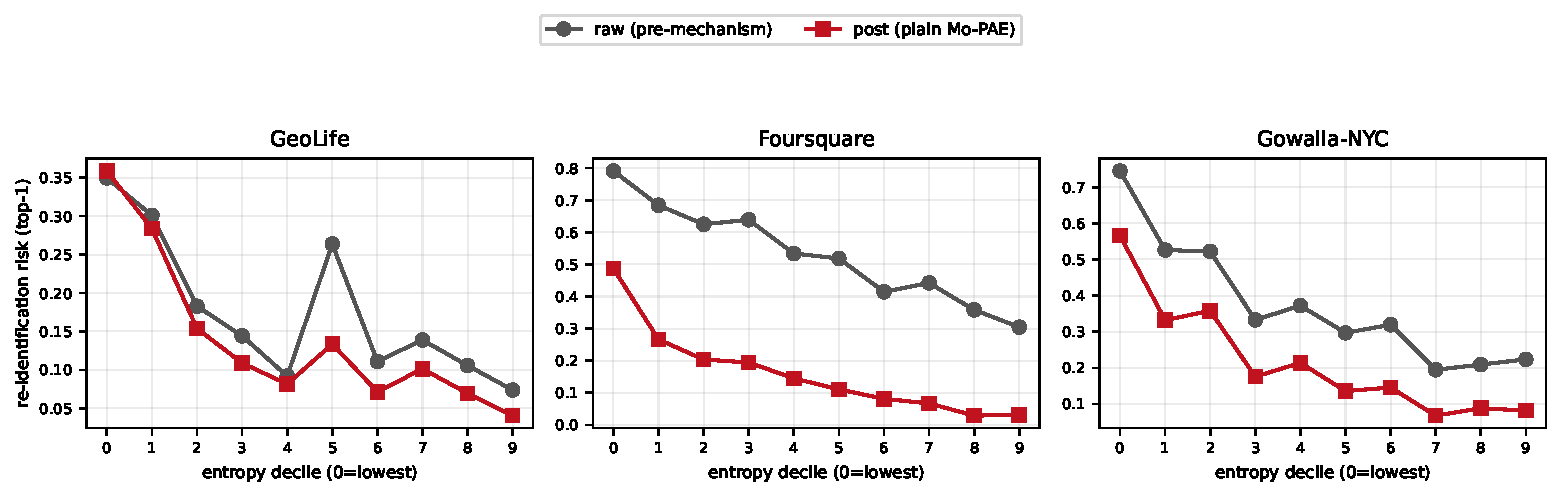
\includegraphics[width=\linewidth]{figures/fig1_raw_vs_post_by_decile.pdf}
\caption{Raw (pre-mechanism) vs.\ post-mechanism (plain Mo-PAE)
re-identification risk by entropy decile, GeoLife, Foursquare, and
Gowalla-NYC. The gap between the two lines narrows toward decile 0 in
every dataset: the most-identifiable decile keeps the largest share of
its original risk.}
\label{fig:raw-vs-post}
\end{figure}

On GeoLife and Foursquare, plain Mo-PAE reliably reduces risk for users
in the middle of the entropy distribution, but gives the lowest-entropy
decile no statistically detectable benefit beyond what a regression on
entropy, radius of gyration, and window count alone would predict --
entropy survives these controls as a significant negative predictor of
post-mechanism risk in every dataset we study (all $p < 10^{-6}$).
Table~\ref{tab:main-disparate-risk} reports the corrected decile-level
metrics (Section~\ref{sec:decile-reduction-metrics}) for these two
datasets plus Gowalla-NYC: on GeoLife, decile 0's relative risk
reduction is not statistically distinguishable from zero while decile
9's is; on Foursquare and Gowalla-NYC, decile 0 does receive a clearly
nonzero reduction, but far less than decile 9's, leaving a residual-risk
disparity ratio of 7--16$\times$ across the three datasets (every CI
excluding $1\times$, i.e.\ no disparity) and an absolute risk gap of
0.3--0.5 between the two deciles.

\begin{table*}[t]
\centering
\caption{Residual-risk disparity under plain Mo-PAE -- ratio (decile 0 $\div$ decile 9) and absolute difference (decile 0 $-$ decile 9) of post-mechanism risk -- and relative risk reduction at deciles 0 and 9, GeoLife, Foursquare, and Gowalla-NYC. Bootstrap 95\% CIs in brackets. Generated from \texttt{reports/figures/paper\_section8/geolife\_foursquare\_disparate\_risk.json}.}
\label{tab:main-disparate-risk}
\small
\begin{tabular}{@{}lccccc@{}}
\toprule
Dataset & $n$ & Rel.\ reduction, decile 0 & Rel.\ reduction, decile 9 & Disparity ratio (0/9) & Disparity difference (0$-$9) \\
\midrule
GeoLife & 178 & -0.032 [-0.189, +0.105] & +0.434 [+0.167, +0.617] & 8.81$\times$ [4.54, 15.16] & 0.318 [0.156, 0.495] \\
Foursquare & 1083 & +0.384 [+0.331, +0.439] & +0.897 [+0.866, +0.925] & 15.54$\times$ [10.84, 23.71] & 0.456 [0.396, 0.519] \\
Gowalla-NYC & 272 & +0.240 [+0.115, +0.371] & +0.634 [+0.519, +0.731] & 6.93$\times$ [4.24, 11.71] & 0.484 [0.336, 0.636] \\
\bottomrule
\end{tabular}
\end{table*}


Table~\ref{tab:gowalla-disparate-risk} reports the same metrics on all
four Gowalla metro subsets. In every one, the relative risk reduction
at the lowest-entropy decile is smaller than at the highest -- in
Gowalla-Chicago's smallest-sample case, the point estimate is slightly
negative, though its CI includes zero -- and the residual-risk
disparity ratio between the two deciles is large and statistically
significant in all four metros (2.2--5.9$\times$, every CI excluding
$1\times$).

\begin{table*}[t]
\centering
\caption{Residual-risk disparity (post-mechanism risk, decile 0 $\div$ decile 9) and relative reduction at deciles 0 and 9, plain Mo-PAE, all four Gowalla metro subsets. Bootstrap 95\% CIs in brackets. Generated from \texttt{reports/figures/phase2d/decile\_reduction\_metrics.json}.}
\label{tab:gowalla-disparate-risk}
\small
\begin{tabular}{@{}lccc@{}}
\toprule
Dataset & Rel.\ reduction, decile 0 & Rel.\ reduction, decile 9 & Residual disparity (0/9) \\
\midrule
Gowalla-NYC & 0.182 [0.116, 0.255] & 0.436 [0.328, 0.540] & 5.85$\times$ [3.87, 8.99] \\
Gowalla-LA & 0.183 [0.073, 0.321] & 0.477 [0.426, 0.529] & 2.23$\times$ [1.25, 3.46] \\
Gowalla-Chicago & -0.010 [-0.182, 0.140] & 0.450 [0.342, 0.547] & 5.40$\times$ [2.62, 9.75] \\
Gowalla-SF-Bay & 0.243 [0.159, 0.335] & 0.564 [0.513, 0.612] & 3.14$\times$ [2.19, 4.30] \\
\bottomrule
\end{tabular}
\end{table*}


A ratio and an absolute difference can disagree in direction whenever
both deciles' risk is falling but the higher-entropy decile's is
falling faster in relative terms -- Section~\ref{sec:residual-risk}
reports a case where this happens, and Table~\ref{tab:main-disparate-risk}
reports both statistics throughout this paper for exactly this reason.

\section{Mo-PAE Residual-Risk Disparity}
\label{sec:residual-risk}

Table~\ref{tab:04d-decile-reduction}'s \emph{plain} and \emph{no-privacy}
rows report, for each dataset, the relative reduction in
re-identification risk (Definition~2) at the lowest- and
highest-entropy deciles, and the residual-risk-disparity ratio
(Definition~3) between them, under plain Mo-PAE's own privacy-utility
trade-off (no fairness term). Table~\ref{tab:inmodel-vs-external}
reports the mechanistic finding from the in-model-vs.-external
comparison described in Section~\ref{sec:methods-changed}.

\begin{table*}[t]
\centering
\caption{Checkpoint 04d: utility, relative risk reduction at deciles 0 and 9, and residual-risk disparity (RRD, post-mechanism risk decile 0 $\div$ decile 9), every approved-batch run. Bootstrap 95\% CIs in brackets; $\geq 3$ encoder seeds per point. Generated from \texttt{reports/figures/phase4d\_analysis/decile\_reduction\_metrics.json}.}
\label{tab:04d-decile-reduction}
\small
\begin{tabular}{@{}llcccc@{}}
\toprule
Dataset & Run & Utility & Rel.\ red., decile 0 & Rel.\ red., decile 9 & RRD (0/9) \\
\midrule
GeoLife & plain Mo-PAE & 0.532$\pm$0.052 & +0.014 [-0.133, +0.176] & +0.371 [-0.042, +0.625] & 8.08 [3.72, 14.11] \\
GeoLife & no-privacy ref. & 0.623$\pm$0.014 & -0.032 [-0.173, +0.104] & +0.340 [-0.045, +0.604] & 8.02 [3.79, 13.93] \\
GeoLife & ed\_soft $\lambda_4$=0.3 & 0.641$\pm$0.039 & +0.160 [+0.016, +0.295] & +0.239 [-0.076, +0.481] & 5.57 [2.67, 9.40] \\
GeoLife & ed\_soft $\lambda_4$=1.0 & 0.654$\pm$0.039 & +0.255 [+0.079, +0.408] & +0.245 [-0.151, +0.516] & 5.00 [2.49, 8.38] \\
GeoLife & ed\_soft $\lambda_4$=3.0 & 0.631$\pm$0.014 & +0.302 [+0.196, +0.419] & +0.299 [-0.019, +0.534] & 5.08 [2.44, 8.76] \\
GeoLife & floor $\lambda_4$=0.3 & 0.551$\pm$0.047 & -0.031 [-0.158, +0.096] & +0.347 [-0.097, +0.614] & 8.19 [3.95, 14.20] \\
GeoLife & floor $\lambda_4$=1.0 & 0.545$\pm$0.055 & -0.010 [-0.154, +0.114] & +0.425 [+0.142, +0.603] & 8.82 [4.56, 14.63] \\
GeoLife & floor $\lambda_4$=3.0 & 0.516$\pm$0.085 & -0.008 [-0.128, +0.111] & +0.473 [+0.210, +0.650] & 9.68 [4.74, 16.43] \\
\addlinespace
Foursquare & plain Mo-PAE & 0.111$\pm$0.005 & +0.384 [+0.331, +0.439] & +0.897 [+0.866, +0.925] & 16.02 [10.84, 23.71] \\
Foursquare & no-privacy ref. & 0.280$\pm$0.002 & +0.096 [+0.065, +0.127] & +0.310 [+0.250, +0.374] & 3.43 [2.74, 4.32] \\
Foursquare & ed\_soft $\lambda_4$=0.3 & 0.134$\pm$0.021 & +0.300 [+0.243, +0.358] & +0.850 [+0.810, +0.885] & 12.38 [8.61, 17.59] \\
Foursquare & ed\_soft $\lambda_4$=1.0 & 0.221$\pm$0.011 & +0.135 [+0.095, +0.179] & +0.600 [+0.543, +0.658] & 5.68 [4.37, 7.38] \\
Foursquare & ed\_soft $\lambda_4$=3.0 & 0.233$\pm$0.004 & +0.133 [+0.096, +0.171] & +0.568 [+0.508, +0.628] & 5.28 [4.10, 6.85] \\
\addlinespace
Gowalla-NYC & plain Mo-PAE & 0.269$\pm$0.035 & +0.240 [+0.115, +0.371] & +0.634 [+0.519, +0.731] & 7.26 [4.24, 11.71] \\
Gowalla-NYC & no-privacy ref. & 0.322$\pm$0.005 & +0.200 [+0.077, +0.343] & +0.334 [+0.245, +0.430] & 4.12 [2.63, 6.27] \\
Gowalla-NYC & ed\_soft $\lambda_4$=0.3 & 0.263$\pm$0.005 & +0.253 [+0.149, +0.360] & +0.555 [+0.452, +0.650] & 5.82 [3.61, 9.08] \\
Gowalla-NYC & ed\_soft $\lambda_4$=1.0 & 0.239$\pm$0.026 & +0.266 [+0.160, +0.381] & +0.596 [+0.527, +0.664] & 6.29 [3.86, 10.02] \\
Gowalla-NYC & ed\_soft $\lambda_4$=3.0 & 0.169$\pm$0.043 & +0.244 [+0.154, +0.345] & +0.629 [+0.540, +0.719] & 7.13 [4.24, 11.69] \\
\addlinespace
\bottomrule
\end{tabular}
\end{table*}

\begin{table}[t]
\centering
\caption{In-model adversary confidence vs.\ external attacker top-1, plain Mo-PAE, deciles 0 and 9. The in-model adversary stays far closer to chance and far flatter across deciles than the external attacker on the identical features. Generated from \texttt{reports/figures/phase4d\_analysis/inmodel\_vs\_external.json}.}
\label{tab:inmodel-vs-external}
\small
\begin{tabular}{@{}lccc@{}}
\toprule
Dataset & Chance & Decile 0 (ext.\ / in-model) & Decile 9 (ext.\ / in-model) \\
\midrule
GeoLife & 0.0055 & 0.345 / 0.0246 & 0.045 / 0.0113 \\
Foursquare & 0.0009 & 0.487 / 0.0521 & 0.031 / 0.0020 \\
Gowalla-NYC & 0.0001 & 0.566 / 0.0776 & 0.082 / 0.0063 \\
\bottomrule
\end{tabular}
\end{table}


\textbf{Plain Mo-PAE gives decile 0 no protection distinguishable from
none, on the dataset where this was checked most carefully.} On
GeoLife, decile 0's relative risk reduction under plain Mo-PAE is not
statistically distinguishable from zero (Table~\ref{tab:main-disparate-risk}),
while decile 9 receives a clearly positive reduction. The
residual-risk-disparity ratio is large: decile 0's post-mechanism
re-identification risk is several times decile 9's. On Foursquare and
Gowalla-NYC, plain Mo-PAE does give decile 0 a clearly nonzero
reduction ($+0.384$ and $+0.240$ respectively, both CIs excluding
zero), but the disparity is still large (residual-risk ratio
$16.02\times$ and $7.26\times$) because decile 9 is reduced far more
($+0.897$ and $+0.634$).

\textbf{A disparity-ratio claim and an absolute-difference claim can
disagree in direction, and this paper reports both for exactly that
reason.} The no-privacy reference (lambdas
$\lambda_1=\lambda_3=\lambda_4=0$, $\lambda_2=1$: an encoder trained for
next-location prediction alone, with no reconstruction or
re-identification adversary) measures the disparity already present in
an undefended learned representation, decoupled from any privacy
objective. On \textbf{Foursquare}, the residual-risk ratio rises
clearly and significantly from the no-privacy baseline to plain Mo-PAE
($3.40\times$, $[2.74,4.32]$, to $15.54\times$, $[10.84,23.71]$ --
non-overlapping CIs), while the absolute difference (decile 0 $-$
decile 9) moves the \emph{opposite} direction, from $0.505$,
$[0.430,0.577]$, to $0.456$, $[0.396,0.519]$ -- overlapping CIs, not
independently significant, but notably not widening either. Decile 0's
own post-mechanism risk drops substantially in absolute terms
($0.715 \to 0.487$). On \textbf{Gowalla-NYC}, neither the ratio
($3.99\times,[2.63,6.27] \to 6.93\times,[4.24,11.71]$) nor the
difference ($0.446,[0.294,0.597] \to 0.484,[0.336,0.636]$) is
statistically distinguishable between the no-privacy baseline and
plain Mo-PAE -- both metrics' confidence intervals overlap
substantially, so ``widens'' is not a safe claim here despite the point
estimates moving upward. On \textbf{GeoLife}, both metrics agree the
two are indistinguishable. The one claim that survives across datasets
is narrower than a single aggregate statistic would suggest:
Foursquare's residual-risk ratio widens clearly and significantly from
the undefended baseline to plain Mo-PAE; nothing else in this
comparison does, by either metric, on any dataset.

\textbf{A fairness term built on the mechanism's own co-trained
adversary targets the wrong decile.} We test this directly with
floor\_loss, a fairness term that penalizes the co-trained
re-identification unit's confidence once it exceeds a threshold. A
threshold set in absolute terms is unreachable if the unit's own
confidence never gets that high: on GeoLife, that confidence stays
within $0.005$--$0.008$ throughout training, regardless of decile,
because the encoder's own adversarial training suppresses it near
chance by construction -- so a fixed, absolute threshold gives the term
exactly zero gradient at every step. Replacing the fixed threshold with
one scaled to the chance level restores a genuinely nonzero gradient.
Table~\ref{tab:04d-decile-reduction}'s floor\_loss rows show what that
restored gradient actually does: decile 0's relative reduction stays
statistically unchanged from plain Mo-PAE at every fairness weight
tested, while decile 9's reduction rises monotonically with the
fairness weight and the residual-risk ratio gets \emph{worse}, not
better. The restored gradient targets whichever user's in-model
confidence crosses the (now chance-relative) threshold first, and
Table~\ref{tab:inmodel-vs-external} shows that is not preferentially
decile 0's users: GeoLife's in-model adversary stays within a narrow
band across all ten deciles (far flatter than the external attacker's
much wider range), so a confidence-threshold term built on it cannot
reliably single out the decile this paper's own evaluation protocol
identifies as worst-off. This is the mechanistic account, not just the
empirical one, of why a loss-based individual-fairness term built on an
in-model adversary struggles to target real re-identification risk.

A leveling-down check (testing, per decile, whether users harmed
relative to plain Mo-PAE at matched utility are disproportionately the
ones already best-protected, with harmed/helped thresholds derived from
a seed-to-seed null rather than a fixed epsilon) found no comparison
in this batch where the harmed rate clears that null -- most likely an
underpowered test given only 3 encoder seeds, not evidence that no such
redistribution is happening; Section~\ref{sec:phase4} reports a
better-powered version of this check (10 encoder seeds) that does find
a real effect at the aggregate (decile-0) level.

\textbf{A ceiling reference is only informative if it is itself trained
to convergence.} Every mechanism in this section uses a fixed training
budget with no early stopping; a per-epoch diagnostic on GeoLife found
all three mechanisms (no-privacy, plain, and the fairness-weighted
variant tested in Section~\ref{sec:phase4}) still rising substantially
partway through that budget, with their relative utility order changing
by the time training is extended. Table~\ref{tab:no-privacy-ceiling}
reports the no-privacy ceiling both at the original budget and once
extended to convergence: the ceiling rises on GeoLife (0.623 $\to$
0.742) but \emph{falls} on Foursquare (0.280 $\to$ 0.214) and
Gowalla-NYC (0.322 $\to$ 0.251) -- both corrected values fit smoothly
into their own dataset's privacy-weight sweep (Section~\ref{sec:phase4}),
so the shorter-budget values were inflated by the no-privacy
objective's faster early convergence, not a regression in the corrected
values.

\begin{table}[t]
\centering
\caption{No-privacy ceiling utility, before (20 epochs, 04d) and after (40 epochs, Checkpoint 04e) correcting for undertraining. Generated from \texttt{reports/figures/phase4e\_analysis/reference\_curve\_comparisons.json}.}
\label{tab:no-privacy-ceiling}
\small
\begin{tabular}{@{}lcc@{}}
\toprule
Dataset & Ceiling @ 20 epochs (stale) & Ceiling @ 40 epochs (corrected) \\
\midrule
GeoLife & 0.623$\pm$0.014 & 0.742$\pm$0.005 \\
Foursquare & 0.280$\pm$0.002 & 0.214$\pm$0.002 \\
Gowalla-NYC & 0.322$\pm$0.005 & 0.251$\pm$0.001 \\
\bottomrule
\end{tabular}
\end{table}


\section{Formulations Under the Naive-Attacker Standard}
\label{sec:phase4}

\draftnote{DRAFT. Results below are from Checkpoint 04d (ed\_soft, with
$\geq 3$ encoder seeds and utility logged for the first time) and
Checkpoint 04c (the five single-encoder-seed formulations: lipschitz,
variance, group-DRO, per-user minimax, group-adversarial, retained from
an earlier round and not part of this round's retraining -- every
point from that grid is flagged with its encoder-seed count where it
appears). See \texttt{reports/04d\_approved\_batch.md} for the full
analysis this section summarizes.}

Every point below is evaluated under the naive/hardened external
attacker (Section~\ref{sec:threat-model-naive}), against plain Mo-PAE
and the no-privacy reference (Section~\ref{sec:residual-risk}) as the
two end-points of the achievable utility range.

\textbf{ed\_soft is the only formulation in this round's retraining
that improves on plain Mo-PAE in the strict sense required by this
paper's dominance bar (both utility and decile-0 risk, beyond both
points' confidence intervals) -- and only on one of three datasets.}
On GeoLife, ed\_soft at $\lambda_4 \in \{1.0, 3.0\}$ has both higher
utility than plain Mo-PAE with non-overlapping confidence intervals
($0.654\pm0.039$ and $0.631\pm0.014$ vs.\ $0.532\pm0.052$) and a
decile-0 relative risk reduction whose CI excludes zero where plain
Mo-PAE's does not (Table~\ref{tab:04d-decile-reduction}). This is the
one case in the batch that survives the dominance bar; every other
(dataset, formulation, $\lambda_4$) point in this section is reported
as a trade-off, not a dominance claim, per the correction applied
after this paper's own Checkpoint 04c draft stated several unverified
dominance claims.

\textbf{On Foursquare, raising ed\_soft's fairness weight makes the
worst-off decile's actual risk \emph{worse}, not better, while utility
rises.} Decile 0's post-mechanism risk increases monotonically with
$\lambda_4$ (from $0.487$ under plain Mo-PAE to $0.554$, $0.684$, and
$0.686$ at $\lambda_4 = 0.3, 1.0, 3.0$), even as the formulation's
reported utility rises from $0.111$ to $0.233$ and its residual-risk-
disparity ratio falls from $16.02\times$ to $5.28\times$
(Table~\ref{tab:04d-decile-reduction}). The disparity narrows because
decile 9 loses protection faster than decile 0 gains any, not because
decile 0 is better protected -- the configuration this paper's
leveling-down check (below) is designed to catch, and exactly the
configuration in which a run's own headline utility and
fairness-loss numbers would read as straightforward progress.
Gowalla-NYC shows a weaker, non-monotonic version of the same
disparity-narrows-without-decile-0-improving pattern, and a
straightforwardly worse operating point at $\lambda_4=3.0$ (utility
falls to $0.169$ with no corresponding privacy gain).

\textbf{Leveling-down check.} Following the protocol established in
Checkpoint 04c (matching a formulation's point to plain Mo-PAE within
$\pm 0.02$ utility, by decile), 40 of 78 attempted comparisons in this
round could be computed; the rest were skipped because $\lambda_4$
moves ed\_soft's utility by more than the $0.02$ tolerance in most
(dataset, $\lambda_4$) pairs -- a limitation of the matching protocol
against this round's data, not a result in itself. Of the 40 computed:
GeoLife's floor\_loss points (Section~\ref{sec:residual-risk}) flag
5--6 of 10 deciles per $\lambda_4$ as leveling down; the single
ed\_soft point that matched tolerance (Gowalla-NYC, $\lambda_4=0.3$)
flags all 10 of 10 deciles as leveling down, with a mean $49.4\%$ of
users harmed relative to plain Mo-PAE at matched utility. Every
comparison that could be run pointed toward leveling down; none
pointed toward lifting the worst-off decile.

\textbf{The five single-encoder-seed formulations (lipschitz,
variance, group-DRO, per-user minimax, group-adversarial) are not
retrained this round.} They are shown alongside plain Mo-PAE and the
no-privacy reference for the first time (Checkpoint 04c could not plot
plain Mo-PAE's utility at all), but every point from this grid carries
a seed-count mismatch (1 encoder seed vs.\ plain's 3) that this paper
does not resolve -- their inclusion here is for visual context, not
for a dominance or leveling-down claim, neither of which this paper
makes for any of the five.

\draftnote{Figures to add once plotting code exists: Pareto-front
scatter plots (utility vs.\ decile-0 risk) per dataset, with plain
Mo-PAE and the no-privacy reference marked as reference points --
currently only the tables above are generated; a scatter figure is a
later addition to \texttt{paper/scripts/generate\_figures.py}, not
blocked on any further data.}

\section{Conclusion}
\label{sec:conclusion}

\draftnote{DRAFT placeholder. Expand once Sections~\ref{sec:residual-risk}
and~\ref{sec:phase4} are filled in -- the current text only restates
the introduction's two findings and should not be treated as final.}

Naive, group-agnostic evaluation of a learned mobility-privacy
mechanism's fairness is unreliable in (at least) two distinct ways we
have shown to be real and measurable, not merely plausible concerns:
the mechanism itself protects users unevenly, worst for the
lowest-entropy, most-identifiable decile (Section~\ref{sec:disparate-risk});
and a previously reported adaptive-adversary result that appeared to
show naive evaluation \emph{additionally} understates risk
asymmetrically does not survive decomposition into its actual causes
(Appendix~\ref{sec:adaptive-appendix}). Together these point toward a
single, narrower, and more defensible claim than ``this mechanism is
unfair'' or ``naive evaluation is meaningless'': individual-fairness
claims about a learned mobility-privacy mechanism must be measured at
the level of who is actually protected, not an aggregate or a naive
per-group average, and the adversary used to measure that protection
must itself be checked for confounds -- a smaller candidate pool or
side information an adversary would not realistically have -- before
its result is attributed to genuine sophistication.


\bibliographystyle{ACM-Reference-Format}
\bibliography{main}

\appendix
\section{Appendix: Adaptive-Attacker Robustness}
\label{sec:adaptive-appendix}

\draftnote{DRAFT. Underlying data and decomposition are final
(Checkpoint 3d, \texttt{reports/03d\_gap\_decomposition.md}); this
section restates it under the PI's relabeling, not as a new analysis.}

An earlier phase of this project asked whether a fairness-aware
adaptive adversary -- one trained and evaluated within a user's true
behavioral decile, with oracle knowledge of that decile -- recovers
substantially more risk than the naive attacker of
Section~\ref{sec:threat-model-naive}. We decompose that adversary's
apparent advantage into three components, computed per user and
bootstrapped over users: (a) naive, the plain attacker;
(b) \emph{external side information about regularity class} -- the
\emph{same} trained naive model, with its output logits masked to only
the user's true decile's candidate users before taking top-1 (no
retraining); (c) specialized, a model trained and tested only on the
true decile's users; (e) realistic, the specialized model from (c) but
routed at test time by a classifier's \emph{predicted} decile (trained
on released features alone) rather than the oracle label.

Table~\ref{tab:gap-decomposition} reports, per dataset, the mean across
all ten deciles of each gap component -- side information $(b-a)$,
specialization $(c-b)$, and the realistic gap $(e-a)$ -- together with
how many of the ten (dataset, decile) cells have a bootstrap CI
excluding zero. Side information alone (b$-$a) is positive and
significant in every single cell across all three datasets: nearly all
of the originally reported ``adaptive adversary'' advantage is
explained by restricting the naive model's candidate pool to the
user's true decile, which requires no attacker sophistication at all.
Specialization (c$-$b) -- actually training a dedicated model once the
candidate pool is already restricted -- is at or below zero in the
large majority of cells, and never reliably positive. Most
importantly, the group-aware attack from released features alone adds
\emph{no risk}: the realistic gap $(e-a)$ is negative in the large
majority of cells across all three datasets, meaning a realistic
adaptive adversary -- one without oracle access to a user's true
behavioral group -- performs no better, and typically worse, than the
naive attacker it was meant to improve on.

\begin{table*}[t]
\centering
\caption{Gap decomposition (Checkpoint 3d): mean of the side-information, specialization, and realistic gap components across all deciles, per dataset, with the count of (dataset, decile) cells whose bootstrap CI excludes zero. Generated from \texttt{reports/figures/phase3d/*/summary.json}.}
\label{tab:gap-decomposition}
\small
\begin{tabular}{@{}lccc@{}}
\toprule
Dataset & Side info.\ (b$-$a) & Specialization (c$-$b) & Realistic (e$-$a) \\
\midrule
GeoLife & +0.166 (10/10 CI excl.\ 0) & -0.030 (3/10 CI excl.\ 0) & -0.041 (9/10 CI excl.\ 0) \\
Foursquare & +0.193 (10/10 CI excl.\ 0) & -0.040 (8/10 CI excl.\ 0) & -0.155 (9/10 CI excl.\ 0) \\
Gowalla-NYC & +0.210 (10/10 CI excl.\ 0) & -0.016 (1/10 CI excl.\ 0) & -0.108 (9/10 CI excl.\ 0) \\
\bottomrule
\end{tabular}
\end{table*}


This finding does not undermine Section~\ref{sec:disparate-risk}'s
disparate-risk result, which depends only on the naive attacker and is
unaffected by any property of the adaptive adversary studied here.

\section{Appendix: Implementation Notes}
\label{sec:implementation-notes}

This appendix collects data-cleaning and windowing details referenced
from Sections~\ref{sec:datasets} and~\ref{sec:evaluation-protocol}.

\subsection{User-id sparsity (Gowalla)}
Gowalla's \texttt{user\_id} values are sparse within each metro subset
(e.g.\ Gowalla-NYC's maximum id is 7,202 for only 1,517 users with any
data, a $4$--$5\times$ inflation). Naively using the maximum id as the
number of classes for a multiclass classifier -- as our
gradient-boosted-tree attacker architecture does -- made that component
of our evaluation pathologically slow (one fit ran over 14 hours
without completing on a 7,202-way problem that is really a 1,517-way
one). We remap user ids to a dense range before any downstream
processing; GeoLife and Foursquare already have dense id spaces and are
unaffected.

\subsection{Window construction}
GeoLife's \texttt{traj\_id} reflects real trip structure, so windows are
built respecting trajectory boundaries (a trajectory is a genuine,
separate trip). Foursquare check-in data has no native trajectory
identifier; synthesizing one from same-calendar-day grouping left only
71 of 1,083 users with even one length-10 window, so we instead build
windows over each user's full chronological check-in sequence within a
split, ignoring the day boundary.

\subsection{Per-dataset window coverage}
\label{sec:coverage-rates}
The per-user minimum filter (Section~\ref{sec:evaluation-protocol})
removes a negligible fraction of GeoLife (1.7\%) and Foursquare (0\%)
users, but a majority of a pooled Gowalla sample. For Gowalla-NYC
specifically, even after shortening the window length from 10 to 5
steps, only 27.9\% of users had the minimum number of test windows our
protocol requires, short of a 50\% target; the other three Gowalla
metros independently fall in the same 24--37\% range. This motivated
treating the four Gowalla metros as separate datasets
(Section~\ref{sec:datasets}) rather than pooling them: doing so gives
2,235 usable users across the four metros combined, where pooling into
one relaxed-filter sample would not have.


\end{document}
